\documentclass[12pt]{article}\usepackage[]{graphicx}\usepackage[]{color}
%% maxwidth is the original width if it is less than linewidth
%% otherwise use linewidth (to make sure the graphics do not exceed the margin)
\makeatletter
\def\maxwidth{ %
  \ifdim\Gin@nat@width>\linewidth
    \linewidth
  \else
    \Gin@nat@width
  \fi
}
\makeatother

\definecolor{fgcolor}{rgb}{0.345, 0.345, 0.345}
\newcommand{\hlnum}[1]{\textcolor[rgb]{0.686,0.059,0.569}{#1}}%
\newcommand{\hlstr}[1]{\textcolor[rgb]{0.192,0.494,0.8}{#1}}%
\newcommand{\hlcom}[1]{\textcolor[rgb]{0.678,0.584,0.686}{\textit{#1}}}%
\newcommand{\hlopt}[1]{\textcolor[rgb]{0,0,0}{#1}}%
\newcommand{\hlstd}[1]{\textcolor[rgb]{0.345,0.345,0.345}{#1}}%
\newcommand{\hlkwa}[1]{\textcolor[rgb]{0.161,0.373,0.58}{\textbf{#1}}}%
\newcommand{\hlkwb}[1]{\textcolor[rgb]{0.69,0.353,0.396}{#1}}%
\newcommand{\hlkwc}[1]{\textcolor[rgb]{0.333,0.667,0.333}{#1}}%
\newcommand{\hlkwd}[1]{\textcolor[rgb]{0.737,0.353,0.396}{\textbf{#1}}}%
\let\hlipl\hlkwb

\usepackage{framed}
\makeatletter
\newenvironment{kframe}{%
 \def\at@end@of@kframe{}%
 \ifinner\ifhmode%
  \def\at@end@of@kframe{\end{minipage}}%
  \begin{minipage}{\columnwidth}%
 \fi\fi%
 \def\FrameCommand##1{\hskip\@totalleftmargin \hskip-\fboxsep
 \colorbox{shadecolor}{##1}\hskip-\fboxsep
     % There is no \\@totalrightmargin, so:
     \hskip-\linewidth \hskip-\@totalleftmargin \hskip\columnwidth}%
 \MakeFramed {\advance\hsize-\width
   \@totalleftmargin\z@ \linewidth\hsize
   \@setminipage}}%
 {\par\unskip\endMakeFramed%
 \at@end@of@kframe}
\makeatother

\definecolor{shadecolor}{rgb}{.97, .97, .97}
\definecolor{messagecolor}{rgb}{0, 0, 0}
\definecolor{warningcolor}{rgb}{1, 0, 1}
\definecolor{errorcolor}{rgb}{1, 0, 0}
\newenvironment{knitrout}{}{} % an empty environment to be redefined in TeX

\usepackage{alltt}
\usepackage{amsmath}
\usepackage{epsfig}
\usepackage{epsf}
\usepackage{graphics}
\usepackage{graphicx}
\usepackage{rotating}
\usepackage{hyperref}
%\usepackage{C:\Program Files\R\R-2.15.0\share\texmf\tex\latex\Sweave}
\usepackage{natbib}
\usepackage{morefloats}
\usepackage{enumitem}
\IfFileExists{upquote.sty}{\usepackage{upquote}}{}
\begin{document}

\begin{center}
{\Large Software Tools for High-Resolution Movement Tags\\
Practical 3}

\bigskip

{\large 9 August 2017}
\bigskip
%\rule{\linewidth}{1mm}
\rule[0cm]{12.7cm}{0.1cm} \vspace{-0.5cm} \tableofcontents
%\rule{\linewidth}{0.5mm}
%\rule[raise-height]{width}{height}
\rule[0cm]{12.7cm}{0.05cm} \vspace{-0.5cm}
\begin{center}
\rule[0cm]{7cm}{0.05cm}
\end{center}

\bigskip
\end{center}



\section{Introduction}
The exercises in this practical will help you explore:
\begin{itemize}
  \item event detection
  \item numerical summaries of events
  \item visualising events
  \item statistical analysis of tag data
  \item inferring behavioural states from tag data
\end{itemize}

The practical contains more exercises than you are likely to be able to complete in the time available, but each section is designed to be relatively stand-alone, so please feel free to pick and choose the topics that are most interesting to you.

Data are provided for each example, but please feel free to try to incorporate your own data as time and ambition allow!

\section{Summarising Dives}
\subsection{Exploring a ready-made dataset}
Consider a dataset on 272 dives by 15 Cuvier's beaked whales. The data were collected using DTAGs, and published along with \cite{DeRuiter2013a}. The data are available from \url{http://dx.doi.org/10.5061/dryad.n77k3}, but we will load a slightly cleaned-up version of the dataset with more manageable variable names.  
\begin{enumerate}
\item If you want practice tidying up the variable names yourself, fetch the original text file from the Dryad repository and get to work.
\item Read in the clean data from the file \texttt{zc\_dives.csv} on your memory stick, or from the url \url{http://www.calvin.edu/~sld33/data/zc\_dives.csv}.  The main dataset has one column of whale IDs which are strings rather than numeric values. If you would prefer not to deal with these in Matlab/Octave, there is a version of the file called zc\_dives\_numeric.csv that omits that column.



\begin{knitrout}
\definecolor{shadecolor}{rgb}{0.969, 0.969, 0.969}\color{fgcolor}\begin{kframe}
\begin{alltt}
\hlstd{zc_dives} \hlkwb{=} \hlkwd{csvread}\hlstd{(}\hlstr{'zc_dives_numeric.csv'}\hlstd{,}\hlnum{1}\hlstd{);}
\end{alltt}
\end{kframe}
\end{knitrout}

\item Create a simple box plot of the whole dataset (one boxplot per column, since each column of the dataset is one dive summary metric).

\begin{knitrout}
\definecolor{shadecolor}{rgb}{0.969, 0.969, 0.969}\color{fgcolor}
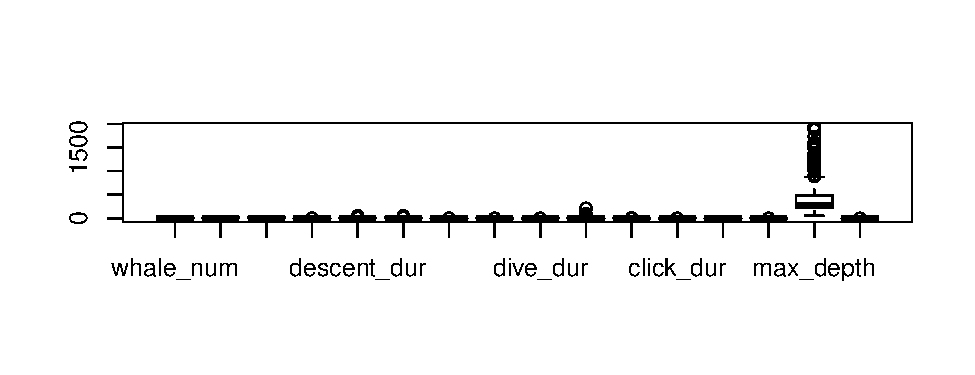
\includegraphics[width=\maxwidth]{figs/real-mdist-simple_boxplot-1} 

\end{knitrout}
\begin{enumerate}
\item What do you notice about the data?
\item How could the visualization be improved (so you can better see patterns in all the variables)? Think creatively and check out the help for the boxplot function for more ideas...
\end{enumerate}

\end{enumerate}%end exploring dive summaries


\bibliographystyle{plainnat} 
\addcontentsline{toc}{section}{References} \bibliography{library} 

\end{document}
